\begin{landscape}
  \section{Mapeamento}
	\subsection{Elementos Válidos}
	\begin{table}[ht]
		\centering
		\begin{tabular}{|m{2cm}|m{2cm}|m{4cm}|m{4cm}|m{7cm}|}
			\hline
			
			\textbf{Número} &
			\textbf{Nome} & 
			\textbf{Descrição} &
			\textbf{Exemplo/Gráfico} &
			\textbf{Exemplo de Codificação} \\
			
			\hline
			
			1 &
			Diagrama de Classes/Classe & 
			Nome, Tipo (Classe, Classe Abstrata, Interface, Enum) &
			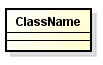
\includegraphics{capitulo08/ClassName.png} & 
			\begin{verbatim}
			public class $ClassName {
			}
			\end{verbatim}
			\\

			\hline
			2 &
			Diagrama de Classes / Atributos & 
			Acessor, tipo e nome &
			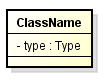
\includegraphics{capitulo08/Type.png} & 
			\begin{verbatim}
			$accessor $Type $type;
			\end{verbatim}
			\\

			\hline
			3 &
			Diagrama de Classes / Cardinalidade & 
			Um para um, um para muitos &
			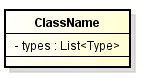
\includegraphics{capitulo08/Collection.png} & 
			\begin{verbatim}
			private $Collection<Type> $type;
			\end{verbatim}
			\\

			\hline
			4 &
			Diagrama de Classes / Construtor & 
			Método público especial com o mesmo nome da classe que tem a responsabilidade de criar uma instância da classe &
			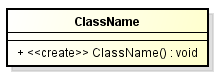
\includegraphics[scale=0.75]{capitulo08/Constructor.png} & 
			\begin{verbatim}
			public $ClassName([$params]);
			\end{verbatim}
			\\
			
			\hline
			5 &
			Diagrama de Classes / Método & 
			Método é uma operação que a classe realiza &
			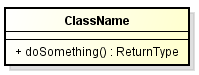
\includegraphics[scale=0.75]{capitulo08/Method.png} & 
			\begin{verbatim}
			$accessor $returnType 
			  $method([$params]);
			\end{verbatim}
			\\
			
			\hline
		\end{tabular}
	\end{table}
	
	\newpage
	
	\subsection{Estruturas Válidas}
	\begin{table}[ht]
		\centering
		\begin{tabular}{|m{2cm}|m{2cm}|m{4cm}|m{5.5cm}|m{5.5cm}|}
			\hline
			
			\textbf{Número} &
			\textbf{Nome} & 
			\textbf{Descrição} &
			\textbf{Sequência / Interligação Gráfico} &
			\textbf{Exemplo de Codificação} \\
			
			\hline
			
			1 &
			Getter & 
			Método acessor para obter valores de um atributo encapsulado em uma classe &
			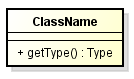
\includegraphics{capitulo08/Getter.png} & 
			\begin{verbatim}
			public $Type get$Type() {
				return this.$type;
			}
			\end{verbatim}
			\\

			\hline
			2 &
			Setter & 
			Método acessor para atribuir valores à um atributo encapsulado em uma classe &
			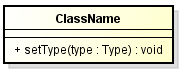
\includegraphics[scale=0.75]{capitulo08/Setter.png} & 
			\begin{verbatim}
			public void set$Type
					($Type $shadowType) {
				this.$type = $shadowType;
			}
			\end{verbatim}
			\\

			\hline
			3 &
			Condicional & 
			A partir de uma condição de guarda o método decide qual direção seguir. &
			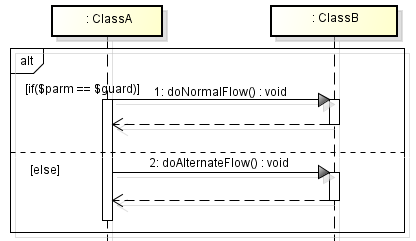
\includegraphics[scale=0.5]{capitulo08/If.png} & 
			\begin{verbatim}
			if($parm == $guard) {
				doNormalFlow();
			} else {
				doAlternateFlow();
			}
			\end{verbatim}
			\\
			
			\hline
		\end{tabular}
	\end{table}
\end{landscape}

\subsection{Regras}
\begin{table}[ht]
	\centering
	\begin{tabular}{|m{2cm}|m{3cm}|m{6cm}|m{4cm}|}
		\hline
		
		\textbf{Número} &
		\textbf{Nome} & 
		\textbf{Descrição} &
		\textbf{Ilustração} \\
			
		\hline
		1 &
		Nome da Classe &
		Nome da classe seguindo o estilo de codificação sa SUN &
		\begin{verbatim}$ClassName\end{verbatim}
		\\

		\hline
		2 &
		Tipo &
		Tipo do atributo&
		\begin{verbatim}$Type\end{verbatim}
		\\

		\hline
		3 &
		Membro &
		Nome do atributo &
		\begin{verbatim}$type\end{verbatim}
		\\

		\hline
		4 &
		Getter &
		Método para obter um valor de um atributo &
		\begin{verbatim}get$Type\end{verbatim}
		\\
			
		\hline
		5 &
		Setter &
		Método para atribuir valores aos atributos &
		\begin{verbatim}set$Type\end{verbatim}
		\\

		\hline
		6 &
		Coleção &
		Coleção de objetos, pode ser mapeada para uma lista ordenada ou um conjunto &
		\begin{verbatim}$Collection\end{verbatim}
		\\

		\hline
		7 &
		Tipo Sombra &
		Parâmetro com o mesmo nome e tipo de um atributo da classe usado para transportar valores para um atributo interno da classe. &
		\begin{verbatim}$shadowType\end{verbatim}
		\\

		\hline
		8 &
		Acessor &
		Tipo de acesso à atributos. Pode assumir: private, public, protected ou "" (default) &
		\begin{verbatim}$accessor\end{verbatim}
		\\
			
		\hline
		9 &
		Método &
		Nome do método &
		\begin{verbatim}$method\end{verbatim}
		\\

		\hline
		10 &
		Lista de Parâmetros &
		Listagem de parâmetros para um método &
		\begin{verbatim}$params\end{verbatim}
		\\

		\hline
		11 &
		Tipo de Retorno &
		Tipo de Retorno que um método pode ter &
		\begin{verbatim}$returnType\end{verbatim}
		\\
		
		\hline
	\end{tabular}
\end{table}
